
\title{Generation of an accurate potential energy surface for carbonylsulfide in helium}
\author{Report on in-depth Practical\\Richard J. M. Beckmann\\Supervisor: Prof. Dominik Marx}
\date{\today}
\documentclass[12pt,titlepage]{article}
\usepackage[english]{babel}
\usepackage[latin1]{inputenc}
\usepackage{color}
\usepackage[a4paper,lmargin={3cm},rmargin={3cm},tmargin={2.5cm},bmargin = {2.5cm}]{geometry}
\usepackage{amssymb}
\usepackage{amsthm}
\usepackage{amsmath}
\usepackage{graphicx}
\usepackage{cite}
\usepackage{textcomp}
\usepackage{gensymb}
\usepackage{float}
\usepackage{subcaption}
\usepackage{caption}
\usepackage{hyperref}
\usepackage{placeins}

\captionsetup[figure]{font={small,it}}
\captionsetup[table]{font={small,it}}
\setlength\parindent{0pt}

\begin{document}
\newcommand{\icm}{\,cm\textsuperscript{-1}}

\begin{titlepage}
	\centering
	\maketitle

\end{titlepage}

\section{Introduction}
\label{introduction}
Helium, the lightest of noble gases, exhibits a number of unsusual properties. It is the only element besides its next-period analogue neon which does not show any chemical reactivity and remains liquid even at 0 K. Instead, it enters a superfluid state, Helium\,II. Characterized at first by its nearly ideal heat conductivity, it was suggested by Kapitza that this was merely an effect of rapid convection caused by the absence of internal friction\cite{Kapitza1938}. This was experimentally shown in 1946 by Elephter Andronikashvili, who measured the moment of inertia of a rod immersed in cold helium. Upon decreasing the temperature the apparent moment of inertia increases until reaching the transition temperature T$_{\lambda}$, below which it would rapidly decrease again. It is assumed that this transition temperature T$_{\lambda}$ marks the onset of superfluidity and that decreasing the temperature converts a growing fraction of the liquid into superfluid helium.
Since superfluidity of \textsuperscript{4}He hinges on bosonic exchange\cite{LONDON1938,Wyatt1998}, it is strictly a cluster effect with no such thing as a single, superfluid helium atom, but emerging from the interaction of a high number of helium atoms. This gives rise to the question of the minimal cluster size necessary to produce this effect. Experimentally, Andronikashvili's experiment can be performed on small clusters by probing the rotational spectrum of single molecules like carbonyl sulfide (OCS)\cite{Grebenev1998} with differing numbers of helium atoms solvating the molecule.\\
To compare these experiments to theoretical predictions and to analyze the physical effects in detail, however, accurate descriptions of the system are required. To use Molecular Dynamics (MD) or Monte Carlo (MC) methods, two of the most common tools to investigate molecular systems, the energy of a given configuration has to be made accessible.{\tiny } The most straightforward way to determine the energy of the molecule and the forces acting on each atom would be an \textit{ab-initio} MD simulation in which a single point electron strucutre calculation is performed after each step. This approach yields highly accurate energies and forces, but it comes at a high computational cost. Paying this high cost is made even more painful by the fact that many configurations are visited more than once, each time calculating repeating the same calculations. A recent solution for this dilemma has arisen in form of neural network potentials (NNPs). These use a machine learning approach to fit a neural network (NN) to a set of known configurations, from which the energy of other configurations can be interpolated. This neural network can then be used to run an MD simulation at very low computational cost while retaining the high accuracy of the method used in its generation.  
\\
\\
In this work, the process of generating, refining and validating a neural network describing OCS solvated in helium will be described. Section \ref{structure} will cover the structure and characteristics of a neural network trained for the prediction of atomic energies. Specifically the use of symmetry functions as input vectors will be discussed.
Then, in section \ref{fitting procedure}, the iterative enhancement of the training set over several generations is described. The NNP acquired in this way was extensively validated as described in section \ref{validation}. Computational details on these processes is given in section \ref{Computational Details}. The manuscript concludes with a summary of the work and an outlook on further investigations in section \ref{summary}. 


\section{High Dimensional Atomic Neural Network Potentials}
\label{structure}
\cite{Behler2007,Behler2011,Behler2015,Behler2017}
An artificial neural network consists three type of layers: The input layer, the output layer and a variable number of hidden layers. The nodes in each layer, the "articifial neurons", are connected with each node in the previous layer and each node in the subsequent layer. The input vector $\underline{I}_{l}$ received by layer $l$ is always a product of the previous layers' $l-1$ output vector $\underline{O}_{l-1}$ and the weight matrix connecting these layers $\underline{\underline{W}}_l$ , modified by an offset vector $\underline{b}_{l}$
\begin{equation}
\label{input value}
\underline{I}_{l} = \underline{b}_{l} + \underline{\underline{W}}_l \cdot \underline{O}_{l-1}
\end{equation}
The exception from this is the input layer, which receives it's values as an input vector that the NN is meant to process.
Additionally, each node may apply some activation function $f_{l, m}$ to the value received to generate it's output value
\begin{equation}
\label{input to output}
\underline{O}_{l} = \underline{f}_{l}(\underline{I}_{l})
\end{equation}
A schematic depiction of a neural network is shown in figure \ref{NN-Beispiel}. 
\newline


\begin{figure}
	\centering
	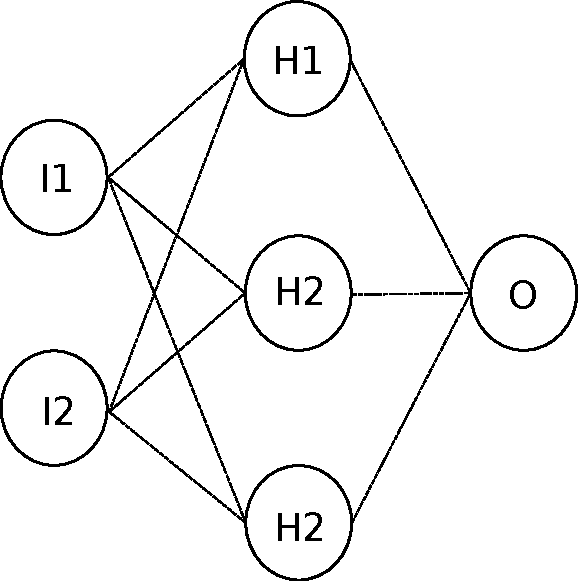
\includegraphics[width=0.6\linewidth]{NN-Beispiel.pdf}
	\caption{Example of a simple neural network. I1 and I2 are the input nodes, H1-H3 the hidden nodes and O the output node. Dashed lines show the connections between nodes.}
	\label{NN-Beispiel}
\end{figure}







\begin{figure}
	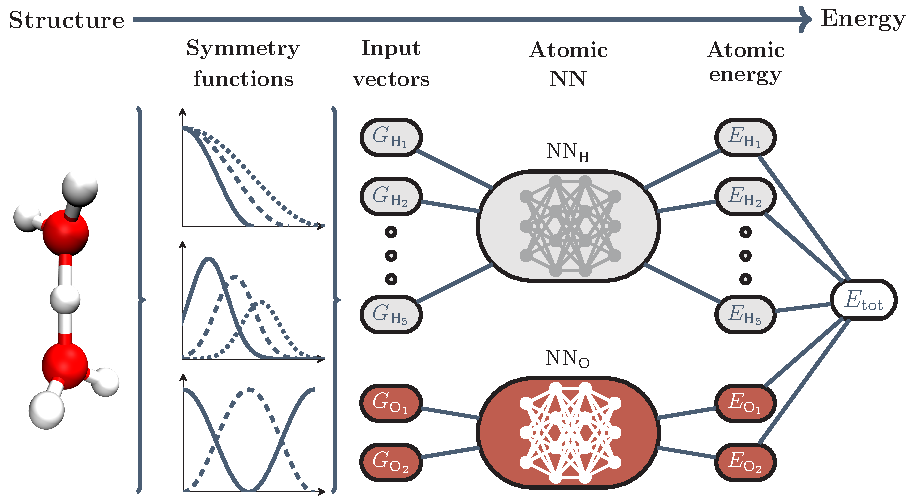
\includegraphics[width=\linewidth]{plot.pdf}
	\caption{Application of a high dimensional atomic neural network potential to a water cluster. The configuration of the system is converted into a description via symmetry functions. These input vectors - one for each atoms in the system - are the fed into the NN specific for the respective atom's element. Thereby an energy output is generated for each atom, the sum of which is the toal energy of the system.}
	\label{application of neural network}
\end{figure}



This basic structure of a feed forward network is adapted for the creation of a high dimensional atomic neural network potential. The total energy of the system in such a network is calculated as a sum of atomic energies which are gained by applying an element specific neural network to each atom. This is schematically shown for a protonated cluster of two water molecules in figure \ref{application of neural network}







Choosing the form of the input vector is one of the most critical choices when creating a NN. In principle, the cartesian coordinates of the system under consideration could be used as input vector from which the neural networks predicts the energy of the system. This, however, comes with several severe drawbacks. For once, the energy of a system is invariant with respect to translation and rotation of the system. This means that, when using cartesian coordinates as input, an ininite number of different inputs will yield the same total energy.
Samewise, the energy must not remain constant if two atoms of the same element are exchanged.\\
To enforce these symmetries, the system with interatomic distances and angles between atoms could be described in intramolecular coordinates. However, if larger systems are to be observed, this would make the use of cut-off radii impossible. since the number of inut functions would vary with the number of atoms within the cut-off radius.
Instead, it has repeatedly been shown to be prudent to use a set of radial and angular symmetry functions for each atom, the value of which depends on the number and position of atoms within the immediate vicinity of the atom under consideration.
The cut-off function is given by:
\begin{equation}
f_C = 
\begin{cases}
0.5 \cdot [cos({\pi R_{ij} \over R_C}) +1] \text{ for $R_{ij} < R_C$}\\
0 \text{ for $R_{ij} > R_C$}
\end{cases}
\end{equation}
where $R_C$ is the cut-off radius and $R_{ij}$ the distance between atoms i and j. In this work, a cut-off radius of $R_C = 12\,\AA$ was chosen.
To describe distances between atoms, radial symmetry functions of the following form were used:
\begin{equation}
G_i^R=\sum_{j \neq i}^{N}e^{-\eta R^2_{ij}} \cdot f_C(R_{ij})
\end{equation} 
where $\eta$ is a parameter manually chosen to modulate the selectivity of the function for atoms at different radii.

The second type of symmetry functions used is the angular symmetry function of the form
\begin{equation}
G_i^\theta = 2^{1-\zeta} \sum_{j \neq i}^N \sum_{k \neq i, j}^{N} (1+\lambda \cos{ \theta_{ijk}})^\zeta e^{\eta (R_{ij}+R_{ik}+R_{jk})^2}\cdot f_C(R_{ij}) \cdot f_C(R_{ik}) \cdot f_C(R_{jk})
\end{equation} 
An overview over all symmetry functions used can be found in table XXX.


\section{Fitting Procedure}
\label{fitting procedure}
To generate a PES for OCS solvated in helium, the potential is split into three parts:
\begin{enumerate}
	\item The intramolecular interaction between oxygen, carbon and sulfur
	\item The intermolecular interaction between helium and OCS
	\item The intermolecular interaction between helium atoms
\end{enumerate}
This splitting is expedient for several reasons:
For once, only the first two of these potentials are described by NNs, whereas the helium-helium interaction can be given by an analytical form \cite{Aziz1995}. This reduces computational cost by a large margin for systems with more than a few helium atoms. Furthermore, this allows the use of the network for different numbers of helium atoms. If the whole system was described with one NN, a new network would have to be fitted everytime the number of atoms is changed.
By this separation of potentials, however, more atoms can be included in the simulation and their interaction energy simply added to the total energy of the system, neglecting only 3-body- and higher interaction terms.

To find a NNP describing the OCS molecule without helium, at first a DFT \textit{ab-initio} trajectory at 300\,K was run. From this trajectory, configurations of the molecule were chosen at random and CCSD(T)-F12a calculations with the AVTZ basis set were performed. Two NNs were trained and tested on these points. As with all NNs created in this work, these NNs possessed two hidden layers with 25 nodes in each layer. To adjust the weights $w_{l,m,l+1,k}$, backpropagation of errors\cite{Rumelhart1986} was used. With only 40 points, phase space is poorly sampled, even for a relatively simple molecule like OCS. Due to the highly flexible nature of NNs, the two networks will disagree strongly on the energy of configurations which lie in these undersampled areas. This can be utilised to identify these areas and systematically add points to the training set. To do so, a large number of configurations were chosen from the trajectory and the energy predicted by both NNs. For the 40 points for which the difference between predictions were strongest, new CCSD(T) calculations were performed and the points added to the training set. By repeating this procedure, several generations with an iteratively increasing training set were built.
 (MAYBE I SHOULD SHOW THE DEVELOPMENT OF THE MEAN SQUARE ERROR AGAINST THE GENERATION?)
Since this training set was still based on only the 300\,K simulation, the NN was used to perform additional simulations with different simulation methods at temperatures between 1\,K and 1000\,K to sample phase space. The parameters used  in these simulations can be found in section \ref{Computational Details}. To combine these NNs into one final network, the final sets of training points from each condition were accumulated and a NN trained on those points.
\newline
The final set of training points acquired under each of those conditions was then used to generate a NN describing the OCS helium interaction. 
A small number of OCS configurations was taken from this set of points and one helium atom was added to the system at a random position. As before, the energy of these configurations was determined via CCSD(T)-F12a and two interaction NNPs were fitted to these points. In subsequent generations, the training set was iteratively and systematically increased. This was achieved in a similar fashion as before by generating a large number of testing points from which the new points were taken. However, the candidate points were not generated via Molecular Dynamics but Monte Carlo simulations, starting from one of the already existing training points. After ccepting the specified number of moves, the NNs are used to predict the interaction energy at those points. A number of points with strongest disagreement are chosen for CCSD(T)-F12a calculations and added to the training set.
After performing this procedure for each of the different conditions, the training sets were combined and a final network fitted to this combined set.



\section{Validation}
\label{validation}
To test the PES generated for OCS, a normal mode analysis was performed. First, the molecule was geometry optimized using a conjugate gradient algorithm using CCSD(T)-F12a calculations and the NNP. The diagonalized Hessian matrix yielded the normal mode frequencies shown in table \ref{normal modes}. The root mean square deviation (RMSD) between the NNP based calculation and the reference calculation is 6.89\,\icm.


\begin{table}
	\label{normal modes}
	\caption{Comparison between the vibrational frequencies of the molecule in the minimum energy configuration according to the NNP and CCSD(T)-F12a reference calculations. The RMSD is 6.89\,\icm}	
	\begin{tabular}{r | r | r}


		NNP & CCSD(T)-F12a & difference\\

		529.50  & 519.76  & 9.74 \\
		529.50	& 519.94  & 9.56 \\
		874.10  & 873.87  & 0.23  \\
		2086.15 & 2084.67 & 1.84 \\
	\end{tabular}

\end{table}


\section{Computational Details}
\label{Computational Details}
\# I would like to put here the computational details so they do not clog up the text in "Fitting the Neural Network", but maybe it would be more straightforward/natural to put them there? What do you think?



\section{Summary and Outlook}
\label{summary}



\FloatBarrier
\bibliography{literature}
\bibliographystyle{unsrt}

\end{document}